\documentclass{standalone}
\usepackage{tikz}
\usetikzlibrary{patterns, positioning}


\begin{document}
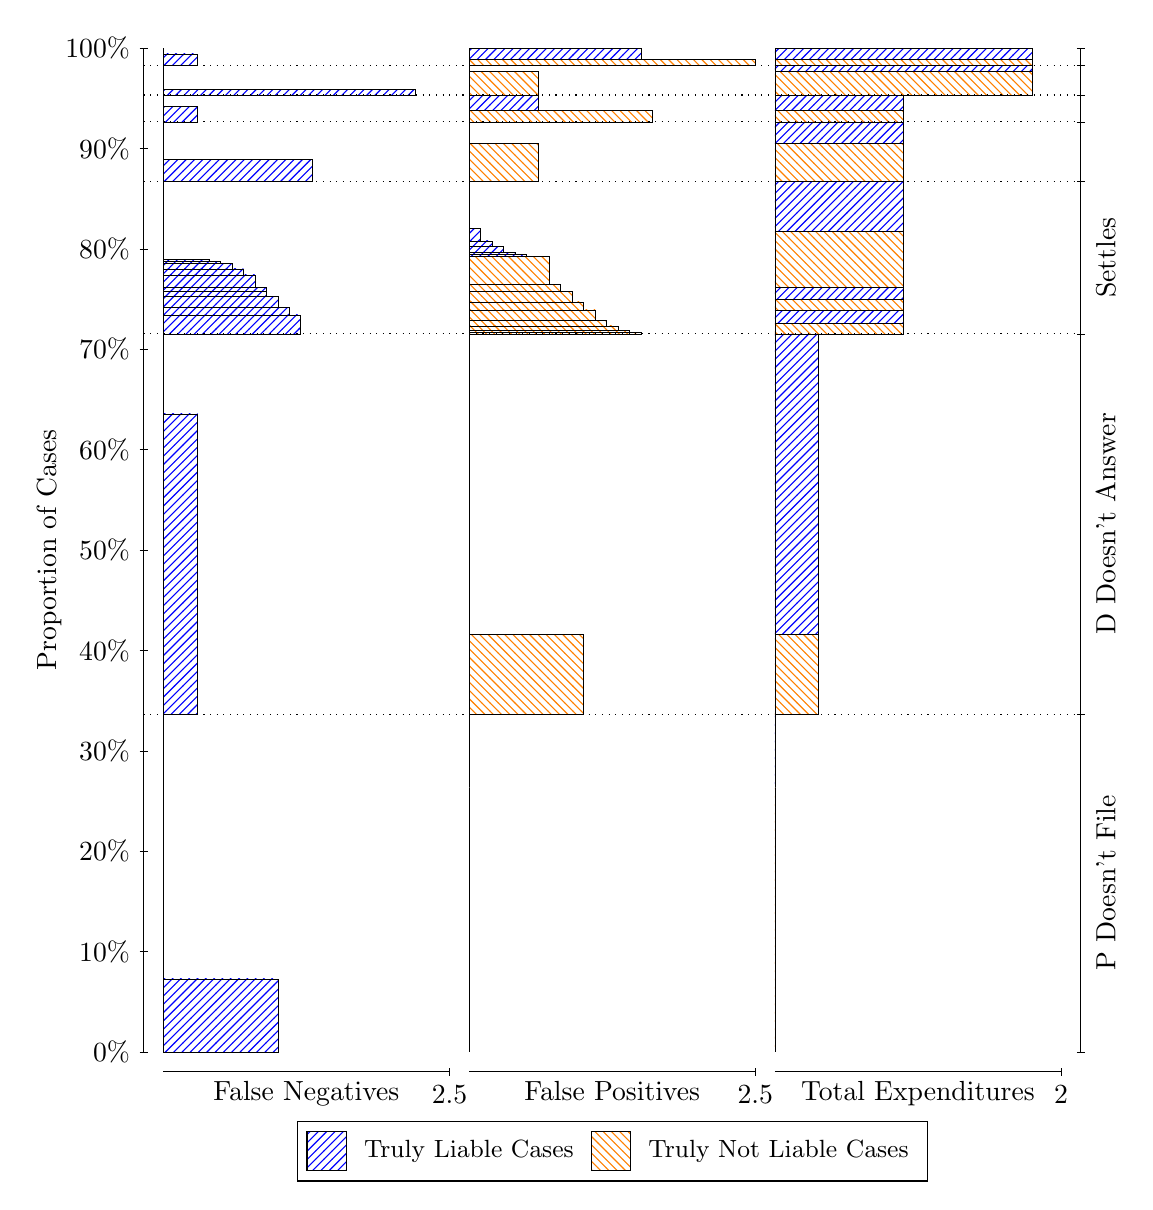
\begin{tikzpicture}
\draw[black, very thin] (1.5,1.75) -- (1.5,14.5);
\node[rotate=90, text=black, anchor=center] at (0.3, 8.125) {Proportion of Cases};
\draw[black, very thin] (1.45,1.75) -- (1.55,1.75);
\node[text=black, anchor=east] at (1.45, 1.75) {0\%};
\draw[black, very thin] (1.45,3.025) -- (1.55,3.025);
\node[text=black, anchor=east] at (1.45, 3.025) {10\%};
\draw[black, very thin] (1.45,4.3) -- (1.55,4.3);
\node[text=black, anchor=east] at (1.45, 4.3) {20\%};
\draw[black, very thin] (1.45,5.575) -- (1.55,5.575);
\node[text=black, anchor=east] at (1.45, 5.575) {30\%};
\draw[black, very thin] (1.45,6.85) -- (1.55,6.85);
\node[text=black, anchor=east] at (1.45, 6.85) {40\%};
\draw[black, very thin] (1.45,8.125) -- (1.55,8.125);
\node[text=black, anchor=east] at (1.45, 8.125) {50\%};
\draw[black, very thin] (1.45,9.4) -- (1.55,9.4);
\node[text=black, anchor=east] at (1.45, 9.4) {60\%};
\draw[black, very thin] (1.45,10.675) -- (1.55,10.675);
\node[text=black, anchor=east] at (1.45, 10.675) {70\%};
\draw[black, very thin] (1.45,11.95) -- (1.55,11.95);
\node[text=black, anchor=east] at (1.45, 11.95) {80\%};
\draw[black, very thin] (1.45,13.225) -- (1.55,13.225);
\node[text=black, anchor=east] at (1.45, 13.225) {90\%};
\draw[black, very thin] (1.45,14.5) -- (1.55,14.5);
\node[text=black, anchor=east] at (1.45, 14.5) {100\%};

\draw[black, very thin] (13.4,1.75) -- (13.4,14.5);
\draw[black, very thin] (13.35,1.75) -- (13.45,1.75);
\node[anchor=west] at (13.35, 1.75) {};
\draw[black, very thin] (13.35,6.0401) -- (13.45,6.0401);
\node[anchor=west] at (13.35, 6.0401) {};
\draw[black, very thin] (13.35,10.869) -- (13.45,10.869);
\node[anchor=west] at (13.35, 10.869) {};
\draw[black, very thin] (13.35,12.803) -- (13.45,12.803);
\node[anchor=west] at (13.35, 12.803) {};
\draw[black, very thin] (13.35,13.563) -- (13.45,13.563);
\node[anchor=west] at (13.35, 13.563) {};
\draw[black, very thin] (13.35,13.903) -- (13.45,13.903);
\node[anchor=west] at (13.35, 13.903) {};
\draw[black, very thin] (13.35,14.281) -- (13.45,14.281);
\node[anchor=west] at (13.35, 14.281) {};
\draw[black, very thin] (13.35,14.5) -- (13.45,14.5);
\node[anchor=west] at (13.35, 14.5) {};

\draw[black, very thin, pattern color=blue, pattern=north east lines] (1.75,1.75) rectangle (3.2033,2.6781);
\draw[black, very thin, pattern color=orange, pattern=north west lines] (1.75,2.6781) rectangle (1.75,6.0401);
\draw[black, very thin, pattern color=blue, pattern=north east lines] (1.75,6.0401) rectangle (2.186,9.8523);
\draw[black, very thin, pattern color=orange, pattern=north west lines] (1.75,9.8523) rectangle (1.75,10.869);
\draw[black, very thin, pattern color=blue, pattern=north east lines] (1.75,10.869) rectangle (3.494,11.11);
\draw[black, very thin, pattern color=blue, pattern=north east lines] (1.75,11.11) rectangle (3.3487,11.204);
\draw[black, very thin, pattern color=blue, pattern=north east lines] (1.75,11.204) rectangle (3.2033,11.348);
\draw[black, very thin, pattern color=blue, pattern=north east lines] (1.75,11.348) rectangle (3.058,11.41);
\draw[black, very thin, pattern color=blue, pattern=north east lines] (1.75,11.41) rectangle (3.058,11.458);
\draw[black, very thin, pattern color=blue, pattern=north east lines] (1.75,11.458) rectangle (2.9127,11.62);
\draw[black, very thin, pattern color=blue, pattern=north east lines] (1.75,11.62) rectangle (2.7673,11.696);
\draw[black, very thin, pattern color=blue, pattern=north east lines] (1.75,11.696) rectangle (2.622,11.766);
\draw[black, very thin, pattern color=blue, pattern=north east lines] (1.75,11.766) rectangle (2.4767,11.794);
\draw[black, very thin, pattern color=blue, pattern=north east lines] (1.75,11.794) rectangle (2.3313,11.814);
\draw[black, very thin, pattern color=orange, pattern=north west lines] (1.75,11.814) rectangle (1.75,12.803);
\draw[black, very thin, pattern color=blue, pattern=north east lines] (1.75,12.803) rectangle (3.6393,13.081);
\draw[black, very thin, pattern color=orange, pattern=north west lines] (1.75,13.081) rectangle (1.75,13.563);
\draw[black, very thin, pattern color=blue, pattern=north east lines] (1.75,13.563) rectangle (2.186,13.755);
\draw[black, very thin, pattern color=orange, pattern=north west lines] (1.75,13.755) rectangle (1.75,13.903);
\draw[black, very thin, pattern color=blue, pattern=north east lines] (1.75,13.903) rectangle (4.9473,13.979);
\draw[black, very thin, pattern color=orange, pattern=north west lines] (1.75,13.979) rectangle (1.75,14.281);
\draw[black, very thin, pattern color=blue, pattern=north east lines] (1.75,14.281) rectangle (2.186,14.425);
\draw[black, very thin, pattern color=orange, pattern=north west lines] (1.75,14.425) rectangle (1.75,14.5);
\draw[black, very thin, pattern color=orange, pattern=north west lines] (5.6333,1.75) rectangle (5.6333,5.112);
\draw[black, very thin, pattern color=blue, pattern=north east lines] (5.6333,5.112) rectangle (5.6333,6.0401);
\draw[black, very thin, pattern color=orange, pattern=north west lines] (5.6333,6.0401) rectangle (7.0867,7.0571);
\draw[black, very thin, pattern color=blue, pattern=north east lines] (5.6333,7.0571) rectangle (5.6333,10.869);
\draw[black, very thin, pattern color=orange, pattern=north west lines] (5.6333,10.869) rectangle (7.8133,10.892);
\draw[black, very thin, pattern color=orange, pattern=north west lines] (5.6333,10.892) rectangle (7.668,10.916);
\draw[black, very thin, pattern color=orange, pattern=north west lines] (5.6333,10.916) rectangle (7.5227,10.97);
\draw[black, very thin, pattern color=orange, pattern=north west lines] (5.6333,10.97) rectangle (7.3773,11.042);
\draw[black, very thin, pattern color=orange, pattern=north west lines] (5.6333,11.042) rectangle (7.232,11.175);
\draw[black, very thin, pattern color=orange, pattern=north west lines] (5.6333,11.175) rectangle (7.0867,11.276);
\draw[black, very thin, pattern color=orange, pattern=north west lines] (5.6333,11.276) rectangle (6.9413,11.406);
\draw[black, very thin, pattern color=orange, pattern=north west lines] (5.6333,11.406) rectangle (6.796,11.494);
\draw[black, very thin, pattern color=orange, pattern=north west lines] (5.6333,11.494) rectangle (6.6507,11.858);
\draw[black, very thin, pattern color=blue, pattern=north east lines] (5.6333,11.858) rectangle (6.36,11.878);
\draw[black, very thin, pattern color=blue, pattern=north east lines] (5.6333,11.878) rectangle (6.2147,11.906);
\draw[black, very thin, pattern color=blue, pattern=north east lines] (5.6333,11.906) rectangle (6.0693,11.976);
\draw[black, very thin, pattern color=blue, pattern=north east lines] (5.6333,11.976) rectangle (5.924,12.052);
\draw[black, very thin, pattern color=blue, pattern=north east lines] (5.6333,12.052) rectangle (5.7787,12.214);
\draw[black, very thin, pattern color=blue, pattern=north east lines] (5.6333,12.214) rectangle (5.6333,12.803);
\draw[black, very thin, pattern color=orange, pattern=north west lines] (5.6333,12.803) rectangle (6.5053,13.285);
\draw[black, very thin, pattern color=blue, pattern=north east lines] (5.6333,13.285) rectangle (5.6333,13.563);
\draw[black, very thin, pattern color=orange, pattern=north west lines] (5.6333,13.563) rectangle (7.9587,13.712);
\draw[black, very thin, pattern color=blue, pattern=north east lines] (5.6333,13.712) rectangle (6.5053,13.903);
\draw[black, very thin, pattern color=orange, pattern=north west lines] (5.6333,13.903) rectangle (6.5053,14.206);
\draw[black, very thin, pattern color=blue, pattern=north east lines] (5.6333,14.206) rectangle (5.6333,14.281);
\draw[black, very thin, pattern color=orange, pattern=north west lines] (5.6333,14.281) rectangle (9.2667,14.356);
\draw[black, very thin, pattern color=blue, pattern=north east lines] (5.6333,14.356) rectangle (7.8133,14.5);
\draw[black, very thin, pattern color=orange, pattern=north west lines] (9.5167,1.75) rectangle (9.5167,5.112);
\draw[black, very thin, pattern color=blue, pattern=north east lines] (9.5167,5.112) rectangle (9.5167,6.0401);
\draw[black, very thin, pattern color=orange, pattern=north west lines] (9.5167,6.0401) rectangle (10.062,7.0571);
\draw[black, very thin, pattern color=blue, pattern=north east lines] (9.5167,7.0571) rectangle (10.062,10.869);
\draw[black, very thin, pattern color=orange, pattern=north west lines] (9.5167,10.869) rectangle (11.152,11.002);
\draw[black, very thin, pattern color=blue, pattern=north east lines] (9.5167,11.002) rectangle (11.152,11.165);
\draw[black, very thin, pattern color=orange, pattern=north west lines] (9.5167,11.165) rectangle (11.152,11.307);
\draw[black, very thin, pattern color=blue, pattern=north east lines] (9.5167,11.307) rectangle (11.152,11.463);
\draw[black, very thin, pattern color=orange, pattern=north west lines] (9.5167,11.463) rectangle (11.152,12.176);
\draw[black, very thin, pattern color=blue, pattern=north east lines] (9.5167,12.176) rectangle (11.152,12.803);
\draw[black, very thin, pattern color=orange, pattern=north west lines] (9.5167,12.803) rectangle (11.152,13.285);
\draw[black, very thin, pattern color=blue, pattern=north east lines] (9.5167,13.285) rectangle (11.152,13.563);
\draw[black, very thin, pattern color=orange, pattern=north west lines] (9.5167,13.563) rectangle (11.152,13.712);
\draw[black, very thin, pattern color=blue, pattern=north east lines] (9.5167,13.712) rectangle (11.152,13.903);
\draw[black, very thin, pattern color=orange, pattern=north west lines] (9.5167,13.903) rectangle (12.787,14.206);
\draw[black, very thin, pattern color=blue, pattern=north east lines] (9.5167,14.206) rectangle (12.787,14.281);
\draw[black, very thin, pattern color=orange, pattern=north west lines] (9.5167,14.281) rectangle (12.787,14.356);
\draw[black, very thin, pattern color=blue, pattern=north east lines] (9.5167,14.356) rectangle (12.787,14.5);
\draw[black, dotted] (1.5,6.0401) -- (13.4,6.0401);
\draw[black, dotted] (1.5,10.869) -- (13.4,10.869);
\draw[black, dotted] (1.5,12.803) -- (13.4,12.803);
\draw[black, dotted] (1.5,13.563) -- (13.4,13.563);
\draw[black, dotted] (1.5,13.903) -- (13.4,13.903);
\draw[black, dotted] (1.5,14.281) -- (13.4,14.281);
\draw[black, very thin] (1.75,1.5) -- (5.3833,1.5);
\node[text=black, anchor=north] at (3.5667, 1.5) {False Negatives};
\draw[black, very thin] (5.3833,1.45) -- (5.3833,1.55);
\node[text=black, anchor=north] at (5.3833, 1.45) {2.5};

\draw[black, very thin] (5.6333,1.5) -- (9.2667,1.5);
\node[text=black, anchor=north] at (7.45, 1.5) {False Positives};
\draw[black, very thin] (9.2667,1.45) -- (9.2667,1.55);
\node[text=black, anchor=north] at (9.2667, 1.45) {2.5};

\draw[black, very thin] (9.5167,1.5) -- (13.15,1.5);
\node[text=black, anchor=north] at (11.333, 1.5) {Total Expenditures};
\draw[black, very thin] (13.15,1.45) -- (13.15,1.55);
\node[text=black, anchor=north] at (13.15, 1.45) {2};

\node[text=black, centered, rotate=90] at (13.72, 3.895) {P Doesn't File};
\node[text=black, centered, rotate=90] at (13.72, 8.4547) {D Doesn't Answer};
\node[text=black, centered, rotate=90] at (13.72, 11.836) {Settles};





\draw (7.449999999999999,1.5) node[draw=none] (baseCoordinate) {};
\begin{scope}[align=center]
        \matrix[scale=0.5, draw=black, below=0.5cm of baseCoordinate, nodes={draw}, column sep=0.1cm]{
            \node[rectangle, draw, minimum width=0.5cm, minimum height=0.5cm, pattern color=blue, pattern=north east lines] {}; &
            \node[draw=none, font=\small, text=black] (B) {Truly Liable Cases}; &
            \node[rectangle, draw, minimum width=0.5cm, minimum height=0.5cm, pattern color=orange, pattern=north west lines] {}; &
            \node[draw=none, font=\small, text=black] (B) {Truly Not Liable Cases}; \\
            };
\end{scope}

\end{tikzpicture}
\end{document}